\section{Dijkstra's Algorithm}

During the development of the ``15-Minute City" algorithm, a number of approaches were considered which were unfeasible in the end. As mentioned earlier in Chapter \ref{algorithms}, All-Source-Shortest-Path algorithms such as Floyd-Warshall's algorithm are not best suited to our problem as it is unnecessary to search from all nodes in the graph. However, another approach to the All-Source-Shortest-Path problem is simply to run Dijkstra's algorithm repeatedly from each node.

Taking inspiration from the approach used by Barbieri et al. (\cite{barbieri_graph_2023}, \ref{barbieri_graph_2023}), the ``15-Minute City" algorithm will use the modified Dijkstra's algorithm to find the 15-Minute City with the service locations of each service type as the source nodes, rather than searching from every vertex in the graph. This approach is expected to be more efficient as the number of service locations is expected to be far smaller than the number of vertices in the graph, $\text{i.e. }S\subset V\Rightarrow|S|<|V|$. Therefore, the first solution proposed in this thesis is a modified version of Dijkstra's algorithm, adapting the methodologies used by Pezzica et al. \cite{cormen2022introduction}, which incorporate the Dijkstra's algorithm with a (Minimum) Priority Queue data structure. The data structure maintains a dynamic set $Q$ of elements, each set element in $Q$ has a key and it supports the following dynamic-set operations.

\begin{itemize}
    \item INSERT($Q; x; k$): inserts element $x$ with key $k$ into set $Q$.
    \item MINIMUM($Q$): returns element of $Q$ with smallest key.
    \item EXTRACT-MIN($Q$): removes and returns element of $Q$ with smallest key.
    \item DECREASE-KEY($Q;x;k$): decreases value of element $x$'s key to $k$. Assumes $k\leq x$'s current key value.
\end{itemize}

All operations take $\mathcal{O}(\log n)$ time in an $n$-element heap with the exception of $\text{MINIMUM}(Q)$ being $\Theta(1)$.

We extend the algorithm so that the algorithm will stop once all nodes within $t$ minutes have been visited. For each node considered in the algorithm, a new label $v.d$ is created where $v.d \in \mathbb{R}_{\geq 0}$ representing the distance from the current source node of the algorithm, initialised to $\infty$.

As the 15-Minute City concept is primarily used to study cities' characteristics, the input graph of the algorithm is expected to be far larger than a single ``15-Minute City". Therefore, it is necessary to stop the algorithm once all nodes within $t$ minutes have been visited to prevent the algorithm from running indefinitely. The modified algorithm is shown in Algorithm \ref{alg:modified_dijsktra}.

\begin{algorithm}[H]
    \caption{Modified Dijkstra's Algorithm} \label{alg:modified_dijsktra}
    \textbf{Input:} A graph $G(V,E)$, weights $w:E\rightarrow\mathbb{R}_{\geq 0}$, source vertex $s$, \\ \phantom{\textbf{Input:}} time threshold $t$ and $i$ denotes the index of the service type\\
    \textbf{Output} Assign $v.r[i]=1$ for vertices that can reach to source node $s$ within threshold $t$ % Set $S$ of vertices reachable by at most $t$ minutes
    \begin{algorithmic}
        \For {each vertex $v\in V$}
            \State $v.d\gets\infty$
        \EndFor
        \State $s.d\gets 0$
        % \State $S\gets\emptyset$
        \State $Q\gets\emptyset$
        \For {each vertex $v\in V$}
            \State INSERT($Q,v$)
        \EndFor
        \While {$Q\neq\emptyset$}
            \State $v\gets$EXTRACT-MIN$(Q)$
            \If {$v.d>t$}
                \State $Q\gets\emptyset$ \Comment{Break out of While loop}
            \Else
                % \State $S\gets S\cup\{v\}$
                \State $v.r[i] \gets 1 $
                \For {each vertex $u\in Adj[v]$}
                    \If {$u.d>v.d+w(u,v)$}
                        \State $u.d\gets v.d+w(u,v)$
                        \State DECREASE-KEY($Q,u,u.d$)
                    \EndIf
                \EndFor
            \EndIf
        \EndWhile
    \end{algorithmic}
\end{algorithm}

The modified Dijkstra's algorithm shown above only searches for vertices within $t$ minutes from a single source node. For our context of the 15-Minute City, this needs to run for each location of each service type. The 15-Minute City algorithm as the solution of the problem is shown in Algorithm \ref{alg:15mc}.

\begin{algorithm}[H]
    \caption{15-Minute City Algorithm}\label{alg:15mc}
    \textbf{Input:} A graph $G(V,E)$, weights $w:E\rightarrow\mathbb{R}_{\geq 0}$, a time threshold $t$ \\ \phantom{\textbf{Input:}} and a list $S$ of service vertices of $p$ types\\
    \textbf{Output} Set $R\subseteq V$ representing the $t$-Minute City
    \begin{algorithmic}
        \ForAll{vertex $v \in V$}
            \State $v.r \gets \{\mathbf{0}\}^{p}$
            \State $v.l \gets \{\mathbf{0}\}^{p}$
        \EndFor
        \ForAll{service $v \in S$}
            \State $v.l[i] \gets 1$ for each service type $i$ which belongs to vertex $v$
        \EndFor
        \For {each service type $i\in\{1,...,p\}$}
            \For {each vertex $s$ where $s.l[i]=1$}
                \State $\text{Modified\_Dijkstra}(G,w,s,t,i)$
            \EndFor
        \EndFor
        \State $R\gets\emptyset$
        \For {each vertex $v\in V$}
            \If {$v.r = \mathbf{1}$}
                \State $R \gets R\cup \{v\}$
            \EndIf
        \EndFor
    \end{algorithmic}
\end{algorithm}

\subsection{Analysis}

The time complexity of the modified Dijkstra's algorithm depends on the following:

\begin{itemize}
    \item Initialisation: $\mathcal{O}(|V|)$
    \item $\text{INSERT}$: $|V|\cdot O(|\text{INSERT}|)=O(|V|\cdot|\text{INSERT}|)$
    \item $\text{EXTRACT-MIN}$: $|V|\cdot O(|\text{EXTRACT-MIN}|)=O(|V|\cdot|\text{EXTRACT-MIN}|)$
    \item $\text{DECREASE-KEY}$: $|E|\cdot O(|\text{DECREASE-KEY}|)=O(|E|\cdot|\text{DECREASE-KEY}|)$
\end{itemize}

The time complexity of the algorithm is also affected by the data structure used to implement the priority queue. A binary heap is a common choice for implementing a priority queue, which has a time complexity of $\mathcal{O}(\log |V|)$ for $\text{INSERT}$, $\text{EXTRACT-MIN}$ and $\text{DECREASE-KEY}$ operations. However, if a Fibonacci heap is used instead, the time complexity of the operations is reduced to $\Theta(1)$, $\mathcal{O}(\log |V|)$ and $\Theta(1)$ respectively.

As the latter two operations in the algorithm dominates the former two operations, the time complexity of algorithm \ref{alg:modified_dijsktra} is $\mathcal{O}((|V|+|E|)\log |V|)$ if a binary heap is implemented. This can be reduced to $\mathcal{O}(|V|\log |V|+|E|)$ if a Fibonacci heap is considered instead.

For the complete 15-Minute City Algorithm \ref{alg:15mc}, the algorithm is run for each location of each service type. Denote $q$ as the maximum number of locations for any service type, the time complexity of the algorithm is $\mathcal{O}(p\cdot q\cdot(|V|\log |V|+|E|))$ if a binary heap is implemented and $\mathcal{O}(p\cdot q\cdot(|V|\log |V|+|E|))$ if a Fibonacci heap is implemented. In both cases, the time complexity consider the size of the entire graph, which could be arbitrarily large when a city or a large area is studied. Due to the fact that the modified Dijkstra's algorithm stops once all nodes within weight $t$ are searched, it is important to note that the actual complexity of the algorithm could be potentially much smaller.

\begin{figure}[H]
    \centering
    \begin{subfigure}{0.5\textwidth}
        \centering
        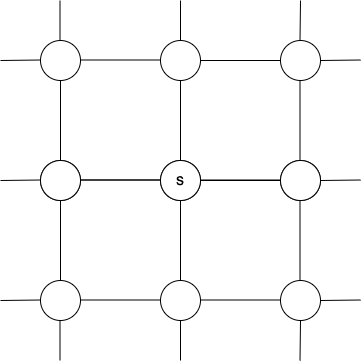
\includegraphics[width=\textwidth]{grid_city.png}
        \caption{Example of a grid city}
        \label{fig:grid_city}
    \end{subfigure}\hfill
    \begin{subfigure}{0.5\textwidth}
        \centering
        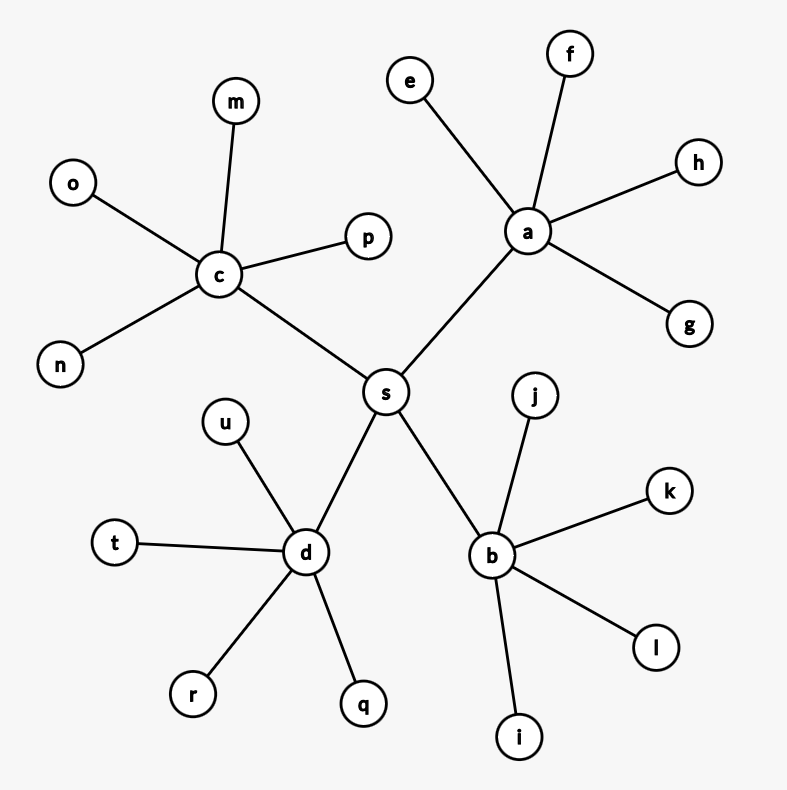
\includegraphics[width=\textwidth]{tree_city.png}
        \caption{Example of a tree city at 2 levels}
        \label{fig:tree_city}
    \end{subfigure}
    % \caption{Three simple graphs}
    % \label{fig:two graphs}
\end{figure}

\subsubsection{Cases where the city is larger than the ``15-Minute City''}

\paragraph{Example}

Consider a city with only square grids and each edge has a weight of 1 (figure \ref{fig:grid_city}). The algorithm will effectively search a total of $1,024$ edges and $545$ nodes for $t=15$. In general, for a grid city (where each node has a degree of 4) given a time threshold $t$, the number of nodes and edges searched by the modified Dijkstra's algorithm can be calculated as follows:

$$
\begin{aligned}
    |\text{Edges}|&=(2\cdot(t+1))^2\\
    |\text{Vertices}|&=1+2\cdot(t+1)\cdot(t+2)
\end{aligned}
$$

This structure of a grid-like city can be applicable to cities such as New York and Barcelona.

\paragraph{Generalisation}

However, if the graph of interest has the following characteristics:

\begin{itemize}
    \item Starting from the source node $s$.
    \item Every node has $d$ successors with $d$ edges of weight 1.
\end{itemize}

An illustration of the graph with 2 levels and $d = 4$ are shown in figure \ref{fig:tree_city}. In this arrangement, given a time threshold $t$ and $d$ the number of nodes branching out from each parent node, the number of nodes and edges need to be visited are as follows:

$$
\begin{aligned}
    |\text{Edges}|&=\sum_{l=1}^{t+1} d^l=d\cdot\left(\frac{1-d^{t+1}}{1-d}\right)\\
    |\text{Vertices}|&=1+|\text{Edges}|
\end{aligned}
$$

For example, setting $t=15$ and $d=4$, the graph will have $|E|=5,726,623,060$ and $|V|=5,726,623,061$.

By limiting the maximum degree for each node in the graph, this graph structure can be considered as the worst case in time complexity for the algorithm with the maximum possible degree of $d+1$ with time threshold $t$. Fixing the degree of the nodes, any other arrangement of the graph (such as a clique) will have an equal or smaller time complexity, as the number of nodes visited will be smaller, and the number of edges unchanged. The time complexity of the modified Dijkstra's algorithm is then:

$$\mathcal{O}(V)=O(\sum_{l=1}^{t+1} d^l)=O(d^{t+1})$$
$$\mathcal{O}(E)=O(1+\sum_{l=1}^{t+1} d^l)=O(d^{t+1})$$

and

$$\mathcal{O}(V\log V+E)=O(d^{t+1}\log d^{t+1}+d^{t+1})=O(d^{t+1}\log d^{t+1})$$

Therefore, the time complexity of the 15-Minute City algorithm on this graph is:

$$\mathcal{O}\left(p\cdot q\cdot d^{t+1}\log d^{t+1}\right)$$

To generalise this notation to edge weights other than 1, define $\epsilon$ as the minimum edge weight in the graph. Then the algorithm can travel at most $\floor*{t/\epsilon}$ edges in $t$ minutes. Therefore, the time complexity of the algorithm can be expressed as:

$$\mathcal{O}\left(p\cdot q\cdot d^{1+\floor*{t/\epsilon}}\log d^{1+\floor*{t/\epsilon}}\right)$$

The space complexity of Dijkstra's algorithm is $\mathcal{O}(|V|+|E|)$. In the modified version of this algorithm, this is simply $\mathcal{O}(d^{1+\floor*{t/\epsilon}}+d^{1+\floor*{t/\epsilon}}) = O(d^{1+\floor*{t/\epsilon}})$. Therefore, the space complexity of the 15-Minute City algorithm on this graph is:

$$\mathcal{O}\left(p\cdot q\cdot d^{1+\floor*{t/\epsilon}}\right)$$

\subsubsection{Cases where the city is smaller than the ``15-Minute City''}

In this case, the city is smaller than the 15-Minute City, the algorithm will search all nodes in the graph. The time complexity of the algorithm is simply just $$\mathcal{O}(|V|\log |V|+|E|)$$

\section{Uniform Cost Search Adaption}

For the space complexity of the proposed algorithm above, it is important to note that the modification algorithm of Dijkstra's algorithm inserts all $|V|$ vertices of the graph into the priority queue set $Q$, this is repeated for each service location of each type. Therefore, the space complexity would be $\mathcal{O}(p\cdot q\cdot |V|)$. Hence the algorithm proposed may not be suitable for large graphs for space complexity.

The problem described here can be solved by adapting a technique from the ``Uniform Cost Search" algorithm. The algorithm is an extension of Best-first search, it is similar to Dijkstra's algorithm, as well as some of the modification to Dijkstra's algorithm we proposed above. However, Uniform Cost Search algorithm does not insert all vertices into the priority queue. Instead, it only inserts the vertices that are reachable within the time threshold $t$. A modification of this algorithm is shown in Algorithm \ref{alg:modified_dijsktra2}. This algorithm can then be used in Algorithm \ref{alg:15mc} to replace the modified Dijkstra's algorithm in \ref{alg:modified_dijsktra}.

\begin{algorithm}[H]
    \caption{Modified Dijkstra's Algorithm 2} \label{alg:modified_dijsktra2}
    \textbf{Input:} A graph $G(V,E)$, weights $w:E\rightarrow\mathbb{R}_{\geq 0}$, source vertex $s$, \\ \phantom{\textbf{Input:}} time threshold $t$ and $i$ denotes the index of the service type\\
    \textbf{Output} Assign $v.r[i]=1$ for vertices that can reach to source node $s$ within threshold $t$ % Set $S$ of vertices reachable by at most $t$ minutes
    \begin{algorithmic}
        \State $Q\gets\emptyset$ \Comment{Initialise an empty priority queue}
        % \State $R\gets\emptyset$ \Comment{Initialise a lookup table for reachable vertices}
        \State INSERT($Q,s$)
        \While {$Q\neq\emptyset$}
            \State $v\gets$EXTRACT-MIN$(Q)$
            \If {$v.d>t$}
                \State $Q\gets\emptyset$ \Comment{Break out of While loop}
            \Else
                \State $v.r[i] \gets 1$
                \For {each vertex $u\in Adj[v]$}
                    \If {$u\notin Q$}
                        \State $u.d\gets v.d+w(u,v)$ % Update reached[u] to v.d+w(u,v)
                        \State INSERT($Q,u$)
                    \ElsIf{$u.d>v.d+w(u,v)$}
                        \State $u.d\gets v.d+w(u,v)$
                        \State DECREASE-KEY($Q,u,u.d$)
                    \EndIf
                \EndFor
            \EndIf
        \EndWhile
    \end{algorithmic}
\end{algorithm}

\subsection{Analysis}

In this implementation, the algorithm is more efficient in practice as it only inserts vertices that are reachable within the time threshold $t$ into the priority queue. However, in the worst case, both time complexity and space complexity remain unchanged.

\section{Inspiration from Johnson's algorithm}

Johnson's algorithm uses both Dijkstra and Bellman-Ford as subroutines and performs better than Floyd-Warshall algorithm in sparse graphs. For the goal of the 15-Minute City algorithm, the set of service vertices can be far smaller than the entire graph in size. Thus, all-pairs shortest path algorithms are not optimal solutions to the problem. However, Johnson's algorithm's approach in connecting multiple nodes with a newly inserted node and $0$ weight can be applied to the 15-Minute City problem.

This approach can be applied to the 15-Minute City problem by adding a new vertex $s$ to the graph and adding edges from the new vertex to all service vertices of the same type. This allows us to eliminate the inner loop of Algorithm \ref{alg:15mc} where $\text{Modified\_Dijkstra}(G, w, s, t, i)$ is called. This alternate approach of the 15-Minute City algorithm is shown in Algorithm \ref{alg:15mc2}.

\begin{algorithm}[H]
    \caption{15-Minute City Algorithm 2} \label{alg:15mc2}
    \textbf{Input:} A graph $G(V,E)$, weights $w:E\rightarrow\mathbb{R}_{\geq 0}$, a time threshold $t$ \\ \phantom{\textbf{Input:}} and a list $S$ of service vertices of $p$ types\\
    \textbf{Output} Set $R\subseteq V$ representing the $t$-Minute City
    \begin{algorithmic}
        \ForAll{vertex $v \in V$}
            \State $v.r \gets \{\mathbf{0}\}^{p}$
            \State $v.l \gets \{\mathbf{0}\}^{p}$
        \EndFor
        \ForAll{service $v \in S$}
            \State $v.l[i] \gets 1$ for each service type $i$ which belongs to vertex $v$
        \EndFor
        \For {each service type $i\in\{1,...,p\}$}
            \State Create a new vertex $s$
            \State Add edges from $s$ to all vertices $v$ where $v.l[i]=1$ and $w(s,v) \gets 0$
            \State $\text{Modified\_Dijkstra\_2}(G,w,s,t,i)$
            \State Remove $s$ and all edges connected to it
        \EndFor
        \State $R\gets\emptyset$
        \For {each vertex $v\in V$}
            \If {$v.r = \mathbf{1}$}
                \State $R \gets R\cup \{v\}$
            \EndIf
        \EndFor
    \end{algorithmic}
\end{algorithm}

\subsection{Analysis}

For each service type, the proposed approach increases the number of vertices by 1 and the number of edges by the number of service vertices of the same type. Denote $q_w$ as the maximum number of vertices of the same service type, then for each service type, Modified\_Dijkstra\_2 algorithm (Algorithm \ref{alg:modified_dijsktra2}) is run, where the algorithm starts from the newly inserted vertex $s$, it visits at most $q_w$ vertices and continues its search as before. The time complexity of the Modified\_Dijkstra\_2 algorithm is then:

$$\mathcal{O}(q_w\cdot(d^{1+\floor*{t/\epsilon}}\log d^{1+\floor*{t/\epsilon}}))=O(d^{1+\floor*{t/\epsilon}}\log d^{1+\floor*{t/\epsilon}})$$

and space complexity:

$$\mathcal{O}(q_w\cdot d^{1+\floor*{t/\epsilon}})=O(d^{1+\floor*{t/\epsilon}})$$

which are the same as before.

However, the time and space complexity of the 15-Minute City algorithm are now:

$$\mathcal{O}\left(p\cdot d^{1+\floor*{t/\epsilon}}\log d^{1+\floor*{t/\epsilon}}\right)\text{ and }O\left(p\cdot d^{1+\floor*{t/\epsilon}}\right)$$

respectively, which are smaller by an order of $q_w$ compared to the previous algorithm.

\section{Adaption to existing papers}

The intuition of our algorithm was inspired by solution approached by Barbieri et al. \cite{barbieri_graph_2023} which we have discussed in Chapter \ref{barbieri_graph_2023}, where we focus on graph searching from services and that we define the 15-Minute City as an interaction of the sets of vertices that can reach to each service type within $t$ minutes, it is easy to see that we can adapt our algorithm into the mathematical notations used by Barbieri et al. In particular, Barbieri et al. denoted

$$C^i=\bigcup\limits_{j=1}^m C^i_j$$

as the nodes that can be reached by $f^i$, where $f^i$ is the set of locations of service type $i$. It is immediately to see the the sets $C^i$ for each service type $i$, is equivalent to the sets of nodes where $v.r[i]=1$. Furthermore, the 15-Minute City $C$ defined by the authors

$$C=\bigcap\limits_{i=1}^n\bigcup\limits_{j=1}^m C^i_j=\bigcap\limits_{i=1}^n C^i\subseteq V$$

is equivalent to our algorithm's output set $R$. Our proposed algorithm focuses on efficiency and computational cost while the approach by Barbieri et al. did not mention the methodology used in calculating the 15-Minute distance. Moreover, Barbieri et al. proposed to use a planar graph. However, it is not clear if a planar graph would be able to represent bridges/tunnels etc effectively, as the definition of a planar graph is that it can be drawn on the plane in such a way that its edges intersect only at their endpoints.

Our algorithm can also be adapted to a number of existing papers which we discussed in Chapter \ref{review}, as most of the work referenced the process of calculating the ``15 minutes'' distance without explicitly laying out the steps taken or methodology used, similar to the paper by Barbieri et al. Notably, Caselli et al. (Section \ref{caselli_exploring_2022}, \cite{caselli_exploring_2022}) defined the ``neighbour cores'' within Parma, Italy and determined the 15-Minute City from these locations. Our algorithm can be adapted to search from these ``neighbour cores'' instead of service locations. 

While Rhoads et al. (Section \ref{rhoads_inclusive_2023}, \cite{rhoads_inclusive_2023}) used a modified Dijkstra's (Egohood) algorithm to compute a 15-Minute City on side-walk networks with a walkability analysis, their work was more focusing on the effect of the percolation analysis on the 15-Minute City (or Egohood by their definition). Their algorithm can be found in the supplementary materials and it is show in Algorithm \ref{alg:egohood}, it is interesting to note that the priority queue used in the Egohood is implemented differently to our Modified Dijkstra's algorithm \ref{alg:modified_dijsktra2}. It is not clear how their priority queue works as the algorithm is not inserting new nodes in the first iteration of the loop.

\begin{algorithm}[H]
    \caption{Egohood Algorithm} \label{alg:egohood}
    \textbf{Input:} A graph $G(V,E)$, weights $w:E\rightarrow\mathbb{R}_{\geq 0}$, source vertex $s$, time threshold $t$ \\
    \textbf{Output} A set $G_s$ containing edges that can be travelled by $s$ within $t$ minutes
    \begin{algorithmic}
        \State $G_s \gets \emptyset$
        \State $s.d\gets 0$
        \For {each vertex $v\in V\setminus\{s\}$}
            \State $v.d\gets\infty$
        \EndFor
        \State $Q\gets\emptyset$
        \State INSERT($Q,s$)
        \While {$Q\neq\emptyset$}
            \State $v\gets$EXTRACT-MIN$(Q)$
            \For {each vertex $u\in Adj[v]$}
                \If {$v.d+w(u,v)\leq t$}
                    \State $G_s\gets G_s\cup\{(u,v)\}$
                    \If {$u\in Q$ and $u.d>v.d+w(u,v)$} \Comment{If $u$ is not visited yet}
                        \State $u.d\gets v.d+w(u,v)$
                        \State INSERT($Q,u$)
                    \EndIf
                \EndIf
            \EndFor
        \EndWhile
    \end{algorithmic}
\end{algorithm}

If there is a typo in the algorithm, where the most inner if statement is actually $$u\notin Q \text{ and }u.d>v.d+w(u,v)$$

The algorithm is not updating the distance of the vertex $u$ if it is already in the priority queue $Q$. However, with this problem fixed, the Egohood algorithm is rather similar to our Modified Dijkstra's algorithm \ref{alg:modified_dijsktra2}.

Lastly, the grid tessellation approaches used by Gaglione et al. (Section \ref{gaglione_urban_2022}, \cite{gaglione_urban_2022}) and Olivari et al. (Section \ref{olivari_are_2023}, \cite{olivari_are_2023}) also involve calculating travelling time between nodes. In particular, the NEXI indices which Olivari et al. have defined requires to search for travlling times between nodes and services as one would in the Graph Representation approach. Thus, our algorithm can be adapted to search for travelling time in such an approach with grid tessellation as well.